\section{eo\-Check\-Point$<$ EOT $>$ Class Template Reference}
\label{classeo_check_point}\index{eoCheckPoint@{eoCheckPoint}}
eo\-Check\-Point is a container class.  


{\tt \#include $<$eo\-Check\-Point.h$>$}

Inheritance diagram for eo\-Check\-Point$<$ EOT $>$::\begin{figure}[H]
\begin{center}
\leavevmode
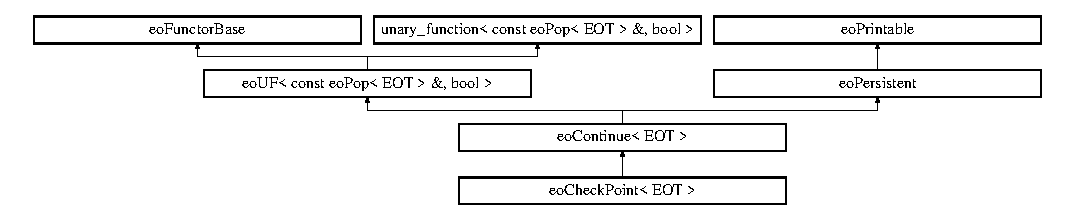
\includegraphics[height=2.52252cm]{classeo_check_point}
\end{center}
\end{figure}
\subsection*{Public Member Functions}
\begin{CompactItemize}
\item 
{\bf eo\-Check\-Point} ({\bf eo\-Continue}$<$ {\bf EOT} $>$ \&\_\-cont)\label{classeo_check_point_a0}

\item 
bool {\bf operator()} (const {\bf eo\-Pop}$<$ {\bf EOT} $>$ \&\_\-pop)\label{classeo_check_point_a1}

\begin{CompactList}\small\item\em The pure virtual function that needs to be implemented by the subclass. \item\end{CompactList}\item 
void {\bf add} ({\bf eo\-Continue}$<$ {\bf EOT} $>$ \&\_\-cont)\label{classeo_check_point_a2}

\item 
void {\bf add} ({\bf eo\-Sorted\-Stat\-Base}$<$ {\bf EOT} $>$ \&\_\-stat)\label{classeo_check_point_a3}

\item 
void {\bf add} ({\bf eo\-Stat\-Base}$<$ {\bf EOT} $>$ \&\_\-stat)\label{classeo_check_point_a4}

\item 
void {\bf add} ({\bf eo\-Monitor} \&\_\-mon)\label{classeo_check_point_a5}

\item 
void {\bf add} ({\bf eo\-Updater} \&\_\-upd)\label{classeo_check_point_a6}

\item 
virtual std::string {\bf class\-Name} (void) const \label{classeo_check_point_a7}

\item 
std::string {\bf all\-Class\-Names} () const \label{classeo_check_point_a8}

\begin{CompactList}\small\item\em returns a string with all class\-Name() of data separated with \char`\"{}$\backslash$n\char`\"{} (for debugging) \item\end{CompactList}\end{CompactItemize}
\subsection*{Private Attributes}
\begin{CompactItemize}
\item 
std::vector$<$ {\bf eo\-Continue}$<$ {\bf EOT} $>$ $\ast$ $>$ {\bf continuators}\label{classeo_check_point_r0}

\item 
std::vector$<$ {\bf eo\-Sorted\-Stat\-Base}$<$ {\bf EOT} $>$ $\ast$ $>$ {\bf sorted}\label{classeo_check_point_r1}

\item 
std::vector$<$ {\bf eo\-Stat\-Base}$<$ {\bf EOT} $>$ $\ast$ $>$ {\bf stats}\label{classeo_check_point_r2}

\item 
std::vector$<$ {\bf eo\-Monitor} $\ast$ $>$ {\bf monitors}\label{classeo_check_point_r3}

\item 
std::vector$<$ {\bf eo\-Updater} $\ast$ $>$ {\bf updaters}\label{classeo_check_point_r4}

\end{CompactItemize}


\subsection{Detailed Description}
\subsubsection*{template$<$class EOT$>$ class eo\-Check\-Point$<$ EOT $>$}

eo\-Check\-Point is a container class. 

It contains std::vectors of (pointers to) {\bf eo\-Continue}{\rm (p.\,\pageref{classeo_continue})} (modif. MS July 16. 2002) eo\-Stats, {\bf eo\-Updater}{\rm (p.\,\pageref{classeo_updater})} and {\bf eo\-Monitor}{\rm (p.\,\pageref{classeo_monitor})} it is an {\bf eo\-Continue}{\rm (p.\,\pageref{classeo_continue})}, so its operator() will be called every generation - and will return the contained-combined-eo\-Continue result but before that it will call in turn every single \{statistics, updaters, monitors\} that it has been given, and after that, if stopping, all last\-Call methods of the above. 



Definition at line 46 of file eo\-Check\-Point.h.

The documentation for this class was generated from the following file:\begin{CompactItemize}
\item 
eo\-Check\-Point.h\end{CompactItemize}
